%!TEX root = report.tex
\exercise{Fourier spectrum}
\setcounter{subsection}{0}
\subsection{Compute Fourier spectrum}
To compute the Fourier spectrum, \textit{MATLAB}'s \texttt{fft2} and \texttt{fftshift} function have been used.
First, the image is transformed to the Fourier domain, using \texttt{fft2}.
Since \texttt{MATLAB} doesn't center the zero-frequency component, but has the zero-frequency component in the corners \cite{fftshift}, \texttt{fftshift} has been used to center the zero-frequency component.

The following function has been used to compute the shifted Fourier spectrum of an image:
\matlabexternal{IPspectrum.m}

\subsection{Display Fourier spectrum}
\begin{figure}[h]
 \centering
 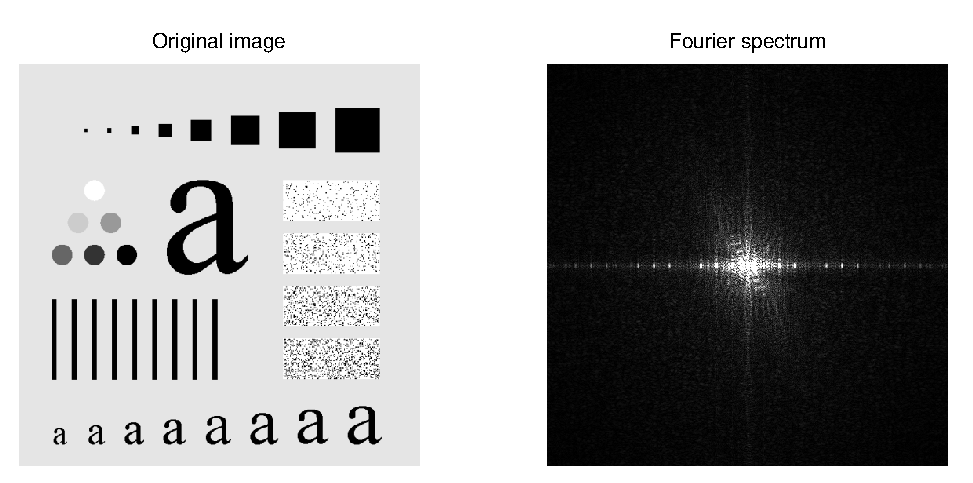
\includegraphics{characters_spectrum.eps}
 \caption{The input image, and the absolute value of its spectrum.}
 \label{fig:characters_spectrum}
\end{figure}

\subsection{Compute average value}
To compute the average value of an image, one could naively sum all pixel values in the spatial domain and divide by the number of pixels.
However, if the image is already available in the Fourier domain, it is more convenient to look at \(F(0, 0)\), i.e., the zero-frequency component.

For the zero-frequenct component, the following holds:
\begin{equation} \label{zero_freq}
\begin{split}
F(0, 0) & = \sum_{x=0}^{M-1}\sum_{y=0}^{N-1}{f(x, y)\mathrm{e}^{0}} \\
 & = \sum_{x=0}^{M-1}\sum_{y=0}^{N-1}{f(x, y)}\text{,} \\
\end{split}
\end{equation}
which is the same as the sum of all pixels in the spatial domain.
Dividing that by the number of pixels yields the average pixel value of the image:
\[\bar{f}(x, y) = \frac{1}{MN}F(0, 0)\]
\clearpage